\documentclass[11pt]{article}
\usepackage[utf8]{inputenc}
\usepackage[dvips]{graphicx}
\usepackage{fancybox}
\usepackage{verbatim}
\usepackage{array}
\usepackage{latexsym}
\usepackage{alltt}
\usepackage{hyperref}
\usepackage{textcomp}
\usepackage{color}
\usepackage{amsmath}
\usepackage{amsfonts}
\usepackage{tikz}
\usepackage{float}
\usepackage[hmargin=3cm,vmargin=5.0cm]{geometry}
%\topmargin=0cm
\topmargin=-2cm
\addtolength{\textheight}{6.5cm}
\addtolength{\textwidth}{2.0cm}
%\setlength{\leftmargin}{-5cm}
\setlength{\oddsidemargin}{0.0cm}
\setlength{\evensidemargin}{0.0cm}


\begin{document}

\section*{Student Information } 
%Write your full name and id number between the colon and newline
%Put one empty space character after colon and before newline
Full Name : Zeynep Özalp \\
Id Number : 2237691 \\

% Write your answers below the section tags
\section*{Answer 1}
\subsection*{a}
Note that the symbol "e" is used as empty string.
\begin{figure}[H]
	\centering
	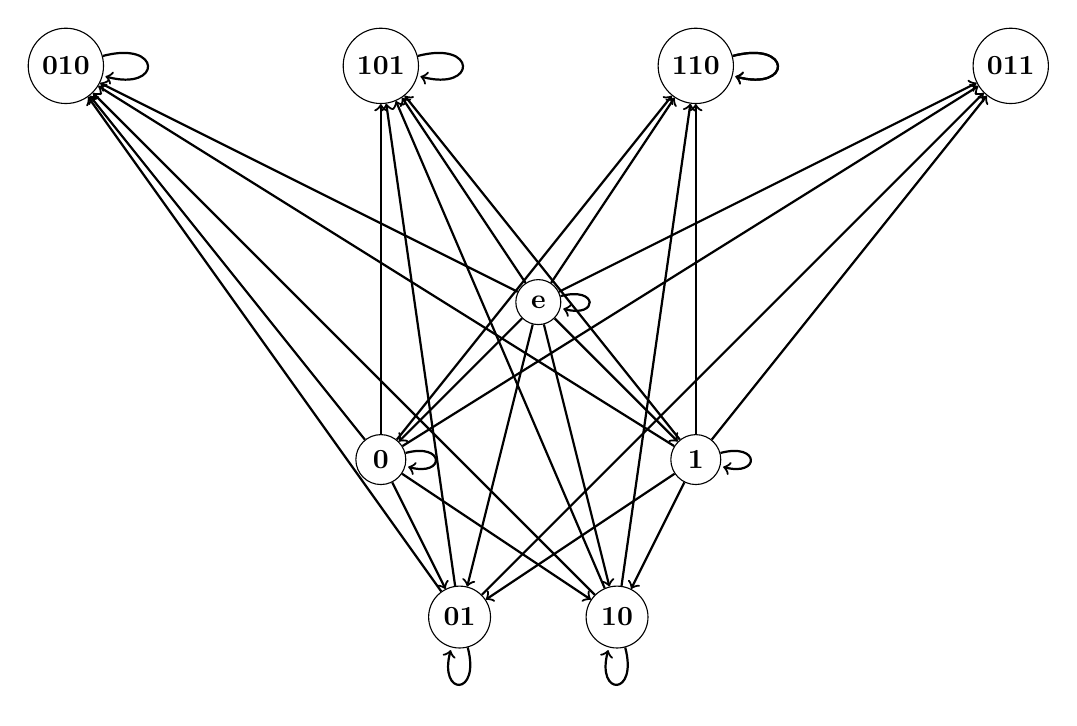
\begin{tikzpicture}
	
	\node[shape=circle,draw=black] (01) at (-1, 0)     {\textbf{01}};
	\node[shape=circle,draw=black] (10) at (1, 0)     {\textbf{10}};
	\node[shape=circle,draw=black] (0) at (-2, 2) 	 {\textbf{0}};
	\node[shape=circle,draw=black] (1) at (2, 2)     {\textbf{1}};
	\node[shape=circle,draw=black] (e) at (0, 4) 	 {\textbf{e}};
	\node[shape=circle,draw=black] (010) at (-6, 7)     {\textbf{010}};
	\node[shape=circle,draw=black] (101) at (-2, 7) 	 {\textbf{101}};
	\node[shape=circle,draw=black] (110) at (2, 7)     {\textbf{110}};
	\node[shape=circle,draw=black] (011) at (6, 7)     {\textbf{011}};
	
	\path[->, thick] (e) edge [loop right] (e);
	\path[->, thick] (e) edge (0);
	\path[->, thick] (e) edge (1);
	\path[->, thick] (e) edge (01);
	\path[->, thick] (e) edge (10);
	\path[->, thick] (e) edge (010);
	\path[->, thick] (e) edge (101);
	\path[->, thick] (e) edge (110);
	\path[->, thick] (e) edge (011);
	\path[->, thick] (0) edge [loop right] (0);
	\path[->, thick] (0) edge (01);
	\path[->, thick] (0) edge (10);
	\path[->, thick] (0) edge (010);
	\path[->, thick] (0) edge (101);
	\path[->, thick] (0) edge (011);
	\path[->, thick] (0) edge (110);
	\path[->, thick] (1) edge [loop right] (1);
	\path[->, thick] (1) edge (01);
	\path[->, thick] (1) edge (10);
	\path[->, thick] (1) edge (010);
	\path[->, thick] (1) edge (101);
	\path[->, thick] (1) edge (110);
	\path[->, thick] (1) edge (011);
	\path[->, thick] (01) edge [loop below] (01);
	\path[->, thick] (01) edge (010);
	\path[->, thick] (01) edge (101);
	\path[->, thick] (01) edge (011);
	\path[->, thick] (10) edge [loop below] (01);
	\path[->, thick] (10) edge (010);
	\path[->, thick] (10) edge (110);
	\path[->, thick] (10) edge (101);
	\path[->, thick] (010) edge [loop right] (010);
	\path[->, thick] (101) edge [loop right] (101);
	\path[->, thick] (110) edge [loop right] (110);
	\path[->, thick] (110) edge [loop right] (011);
	
	\end{tikzpicture} 	
\end{figure}
\subsection*{b}
Since every string is a subset of itself, this relation is reflexive on S. Assume that $aRb$ and $bRa$ for $a,b \in S$. This is possible if and only if $a=b$. So, R is antisymmetric. Clearly, $aRb \wedge bRc \rightarrow aRc$ for $a,b,c \in S$ since if a is a substring of b and b is a substring of c, a is a substring of c. Thus, $(S,R)$ is a poset. 
\subsection*{c}
For every $a,b \in S$, if $a\alpha b$ then the relation $\alpha$ is a total order. For example, between $010$ and $110$ there is no relation. Thus, R is not a total order.
\subsection*{d}
\begin{figure}[H]
	\centering
	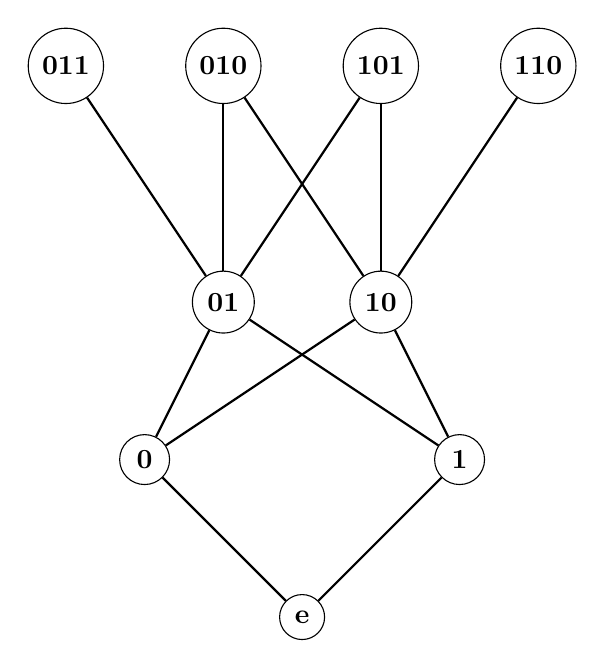
\begin{tikzpicture}
	
	\node[shape=circle,draw=black] (e) at (0, 0)     {\textbf{e}};
	\node[shape=circle,draw=black] (0) at (-2, 2) 	 {\textbf{0}};
	\node[shape=circle,draw=black] (1) at (2, 2)     {\textbf{1}};
	\node[shape=circle,draw=black] (01) at (-1, 4) 	 {\textbf{01}};
	\node[shape=circle,draw=black] (10) at (1, 4) 	 {\textbf{10}};
	\node[shape=circle,draw=black] (101) at (1, 7)     {\textbf{101}};
	\node[shape=circle,draw=black] (010) at (-1, 7) 	 {\textbf{010}};
	\node[shape=circle,draw=black] (011) at (-3, 7)     {\textbf{011}};
	\node[shape=circle,draw=black] (110) at (3, 7)     {\textbf{110}};

	\path[-, thick] (e) edge (0);
	\path[-, thick] (e) edge (1);
	\path[-, thick] (0) edge (01);
	\path[-, thick] (1) edge (01);
	\path[-, thick] (0) edge (10);
	\path[-, thick] (1) edge (10);
	\path[-, thick] (01) edge (010);
	\path[-, thick] (01) edge (101);
	\path[-, thick] (01) edge (011);
	\path[-, thick] (10) edge (110);
	\path[-, thick] (10) edge (010);
	\path[-, thick] (10) edge (101);
	
	\end{tikzpicture} 	
\end{figure}
Minimal: e. Maximal: 010,101,110.
\subsection*{e}
Not a lattice since least upper bound of 010 and 101 does not exist in S.
\section*{Answer 2}
\subsection*{a}
\begin{table}[H]
\small
\centering
\begin{tabular}
{|c|c|}	%% specify column number and vertical lines
\hline
Initial Vertex & Terminal Vertex \\
\hline
a & a,b,d\\
b & c,d\\
c & b\\
d & c\\
e & b,f\\
f & b,e,f\\
g & c,f\\
\hline

\end{tabular}
\end{table}
\subsection*{b}
Order of the vertices is a,b,c,d,e,f,g.
$$
\begin{bmatrix}
1 & 1 & 0 & 1 & 0 & 0 & 0 \\
0 & 0 & 1 & 1 & 0 & 0 & 0 \\
0 & 1 & 0 & 0 & 0 & 0 & 0 \\
0 & 0 & 1 & 0 & 0 & 0 & 0 \\
0 & 1 & 0 & 0 & 0 & 1 & 0 \\
0 & 1 & 0 & 0 & 1 & 1 & 0 \\
0 & 0 & 0 & 0 & 1 & 1 & 0 \\
\end{bmatrix}
$$
\subsection*{c}
\begin{table}[H]
\small
\centering
\begin{tabular}
{|c|c|c|}	%% specify column number and vertical lines
\hline
Vertex & Indegrees & Outdegrees \\
\hline
a & 1 & 3\\
b & 3 & 1\\
c & 3 & 1\\
d & 2 & 1\\
e & 2 & 1\\
f & 2 & 3\\
g & 0 & 2\\
\hline

\end{tabular}
\end{table}
\subsection*{d}
1. abcbd\\
2. adcbc\\
3. ebdcb\\
4. efbdc\\
5. gfebd\\
6. gfbdc
\subsection*{e}
1. dcbd\\
2. bdcb\\
3. cbdc\\
4. feff
\subsection*{f}
Graph G is weakly connected if and only if there is a path between every two vertices when the directions of the edges are disregarded. Vertex b is connected to all vertices except g but vertex g is connected to f and c. Clearly, there is a path between every two vertices.
\subsection*{g}
1. Vertex a.\\
2. Vertex g.\\
3. Subgraph consisting vertices b,c,d and edges (b,c), (c,b), (d,c), (b,d).\\
4. Subgraph consisting vertices e, f and edges (e,f), (f,e). 
\subsection*{h}
1. Between a and b: adcb, abcb.\\
1. Between a and c: aabc, aadc, abdc.\\
2. Between a and d there is 1 path : aabd.\\
3. Between b and d there is 1 path : bcbd.\\
4. Between d and c there is 1 path : dcbc.\\
Total = 8.
\section*{Answer 3}
\subsection*{a}
Theorem in lecture notes of section 3: A graph has a Euler path if it is connected and there is either 0 or 2 vertices of odd degree. Clearly, the graph is connected.\\
deg(a)=2, deg(b)=6, deg(c)=4, deg(d)=4, deg(e)=6, deg(f)=6, deg(g)=4, deg(h)=4, deg(i)=4, deg(j)=6. \\
Therefore, G has a Euler path.
\subsection*{b}
Since the graph is connected and every vertex has a even degree, the graph has an Euler circuit by Theorem 1 on page 696.
\subsection*{c}
One example of Hamiltonian path of G: abfehicdgkj. So, G has a Hamiltonian path.
\subsection*{d}
The number of vertices is 11. Not all of vertices have a degree greater than 11/2 and the greatest number of sum of the degrees of two non adjacent vertices is 10. So, there is no Hamiltonian circuit with respect to Theorem 3 and 4 on page 701.
\section*{Answer 4}
\subsection*{a}
There are m+n vertices. Let use the symbols M and N to represent disjoint sets of m and n vertices, respectively. For each vertex in M, there is an n edges to every vertex in N. Since there are m vertices in M, the number of edges is m times n in total.
\subsection*{b}
Since there is no edge between the elements of M and N, the Hamiltonian path have a zigzag shape.\\

1. Assume that $n>m$\\
a) Assume we begin with a vertex in N. Then, we have to visit a vertex in M, then in N, and goes like a zigzag shape until there are n-m unvisited vertices in N. Since there are no edges between these vertices, there are no Hamiltonian circuit or path.\\
b) Assume we begin with a vertex in M. Again we have a zigzag shape. Since we begin with a vertex in M, path will end at one of vertex in N but there are still n-m unvisited vertices in N. Since there are no edges between these vertices, there are no Hamiltonian circuit or path.\\

2. Assume that $m>n$.\\
a) Assume we begin with a vertex in M. Again we have a zigzag shape. Since we begin with a vertex in M, path will end at one of vertex in N but there are still m-n unvisited vertices in M. Since there are no edges between these vertices, there are no Hamiltonian circuit or path.\\
a) Assume we begin with a vertex in N. Again we have a zigzag shape. There remains m-n unvisited vertices in M. Since there are no edges between these vertices, there are no Hamiltonian circuit or path.\\

\section*{Answer 5}
\subsection*{a}
The table shows visited vertices, selected vertex in each step and current distances of vertices to vertex s. The distances are initially infinity. Distance from s to s is zero (no need to show).
\begin{table}[H]
\small
\centering
\begin{tabular}
{|c|c|c|c|c|c|c|c|c|}	%% specify column number and vertical lines
\hline
Visited Vertices & Selected Vertex & u & v & w & x & y & z & t \\
\hline
  & s & 4 & 5 & 3 & $\infty$ & $\infty$ & $\infty$ & $\infty$ \\
  \hline
 s & w & 4 & 5 & 3 & 11 & $\infty$ & 15 & $\infty$ \\
 \hline
 s, w & u & 4 & 5 & 3 & 11 & 15 & 15 & $\infty$ \\
 \hline
 s, w, u & v & 4 & 5 & 3 & 7 & 11 & 15 & $\infty$ \\
 \hline
 s, w, u, v & x & 4 & 5 & 3 & 7 & 8 & 13 & $\infty$ \\
 \hline
 s, w, u, v, x & y & 4 & 5 & 3 & 7 & 8 & 12 & 17 \\
 \hline
 s, w, u, v, x, y & z & 4 & 5 & 3 & 7 & 8 & 12 & 15 \\
 \hline
 s, w, u, v, x, y, z & t & 4 & 5 & 3 & 7 & 8 & 12 & 15 \\
\hline

\end{tabular}
\end{table}
Shortest path from s to t is svxyzt and its weight is 15.
\subsection*{b}

The root is x. Add y since its weight is minimal, 1.
\begin{figure}[H]
\centering
	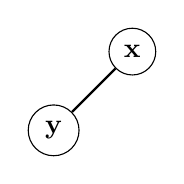
\begin{tikzpicture}
	
	\node[shape=circle,draw=black] (x) at (0, 0)     {\textbf{x}};
	\node[shape=circle,draw=black] (y) at (-1, -1) 	 {\textbf{y}};

	\path[-, thick] (x) edge (y);
	
	
	\end{tikzpicture} 	
\end{figure}

Now, we have vertices x and y. Add v since its weight is smallest among u, w, z, t.
\begin{figure}[H]
\centering
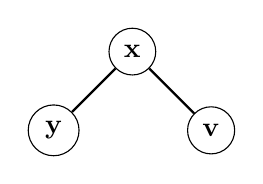
\begin{tikzpicture}
	
	\node[shape=circle,draw=black] (x) at (0, 0)     {\textbf{x}};
	\node[shape=circle,draw=black] (y) at (-1, -1) 	 {\textbf{y}};
	\node[shape=circle,draw=black] (v) at (1, -1) 	 {\textbf{v}};

	\path[-, thick] (x) edge (y);
	\path[-, thick] (x) edge (v);

\end{tikzpicture}
\end{figure}
Now we have vertices x, y and v. Add w since its weight is smallest. This procedure goes like this.
\begin{figure}[H]
\centering
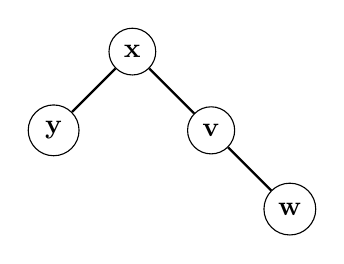
\begin{tikzpicture}
	
	\node[shape=circle,draw=black] (x) at (0, 0)     {\textbf{x}};
	\node[shape=circle,draw=black] (y) at (-1, -1) 	 {\textbf{y}};
	\node[shape=circle,draw=black] (v) at (1, -1) 	 {\textbf{v}};
	\node[shape=circle,draw=black] (w) at (2, -2) 	 {\textbf{w}};

	\path[-, thick] (x) edge (y);
	\path[-, thick] (x) edge (v);
	\path[-, thick] (v) edge (w);

\end{tikzpicture}
\end{figure}

\begin{figure}[H]
\centering
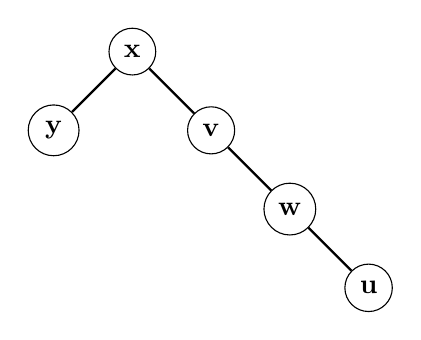
\begin{tikzpicture}
	
	\node[shape=circle,draw=black] (x) at (0, 0)     {\textbf{x}};
	\node[shape=circle,draw=black] (y) at (-1, -1) 	 {\textbf{y}};
	\node[shape=circle,draw=black] (v) at (1, -1) 	 {\textbf{v}};
	\node[shape=circle,draw=black] (w) at (2, -2) 	 {\textbf{w}};
	\node[shape=circle,draw=black] (u) at (3, -3) 	 {\textbf{u}};

	\path[-, thick] (x) edge (y);
	\path[-, thick] (x) edge (v);
	\path[-, thick] (v) edge (w);
	\path[-, thick] (w) edge (u);

\end{tikzpicture}
\end{figure}

\begin{figure}[H]
\centering
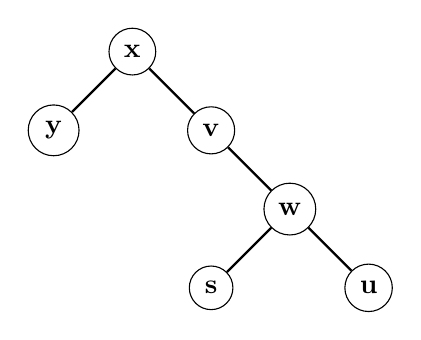
\begin{tikzpicture}
	
	\node[shape=circle,draw=black] (x) at (0, 0)     {\textbf{x}};
	\node[shape=circle,draw=black] (y) at (-1, -1) 	 {\textbf{y}};
	\node[shape=circle,draw=black] (v) at (1, -1) 	 {\textbf{v}};
	\node[shape=circle,draw=black] (w) at (2, -2) 	 {\textbf{w}};
	\node[shape=circle,draw=black] (u) at (3, -3) 	 {\textbf{u}};
	\node[shape=circle,draw=black] (s) at (1, -3) 	 {\textbf{s}};
	
	\path[-, thick] (x) edge (y);
	\path[-, thick] (x) edge (v);
	\path[-, thick] (v) edge (w);
	\path[-, thick] (w) edge (u);
	\path[-, thick] (w) edge (s);

\end{tikzpicture}
\end{figure}

\begin{figure}[H]
\centering
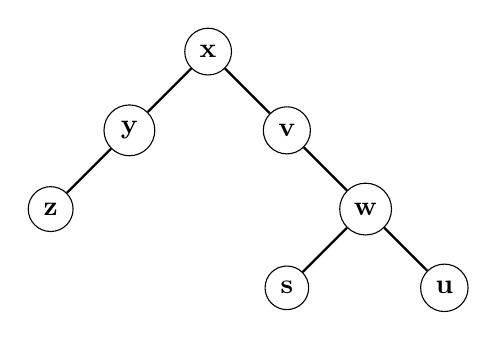
\begin{tikzpicture}
	
	\node[shape=circle,draw=black] (x) at (0, 0)     {\textbf{x}};
	\node[shape=circle,draw=black] (y) at (-1, -1) 	 {\textbf{y}};
	\node[shape=circle,draw=black] (v) at (1, -1) 	 {\textbf{v}};
	\node[shape=circle,draw=black] (w) at (2, -2) 	 {\textbf{w}};
	\node[shape=circle,draw=black] (u) at (3, -3) 	 {\textbf{u}};
	\node[shape=circle,draw=black] (s) at (1, -3) 	 {\textbf{s}};
	\node[shape=circle,draw=black] (z) at (-2, -2) 	 {\textbf{z}};
	
	\path[-, thick] (x) edge (y);
	\path[-, thick] (x) edge (v);
	\path[-, thick] (v) edge (w);
	\path[-, thick] (w) edge (u);
	\path[-, thick] (w) edge (s);
	\path[-, thick] (z) edge (y);

\end{tikzpicture}
\end{figure}

\begin{figure}[H]
\centering
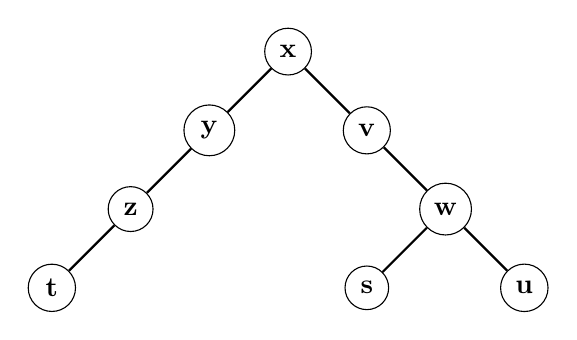
\begin{tikzpicture}
	
	\node[shape=circle,draw=black] (x) at (0, 0)     {\textbf{x}};
	\node[shape=circle,draw=black] (y) at (-1, -1) 	 {\textbf{y}};
	\node[shape=circle,draw=black] (v) at (1, -1) 	 {\textbf{v}};
	\node[shape=circle,draw=black] (w) at (2, -2) 	 {\textbf{w}};
	\node[shape=circle,draw=black] (u) at (3, -3) 	 {\textbf{u}};
	\node[shape=circle,draw=black] (s) at (1, -3) 	 {\textbf{s}};
	\node[shape=circle,draw=black] (z) at (-2, -2) 	 {\textbf{z}};
	\node[shape=circle,draw=black] (t) at (-3, -3) 	 {\textbf{t}};
	
	\path[-, thick] (x) edge (y);
	\path[-, thick] (x) edge (v);
	\path[-, thick] (v) edge (w);
	\path[-, thick] (w) edge (u);
	\path[-, thick] (w) edge (s);
	\path[-, thick] (z) edge (y);
	\path[-, thick] (z) edge (t);

\end{tikzpicture}
\end{figure}
\subsection*{c}
\begin{itemize}
\item After adding (s,x,1):
\begin{figure}[H]
\centering
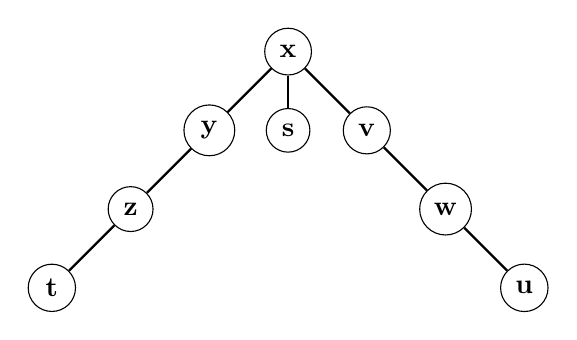
\begin{tikzpicture}
	
	\node[shape=circle,draw=black] (x) at (0, 0)     {\textbf{x}};
	\node[shape=circle,draw=black] (y) at (-1, -1) 	 {\textbf{y}};
	\node[shape=circle,draw=black] (s) at (0, -1) 	 {\textbf{s}};
	\node[shape=circle,draw=black] (v) at (1, -1) 	 {\textbf{v}};
	\node[shape=circle,draw=black] (w) at (2, -2) 	 {\textbf{w}};
	\node[shape=circle,draw=black] (u) at (3, -3) 	 {\textbf{u}};
	\node[shape=circle,draw=black] (z) at (-2, -2) 	 {\textbf{z}};
	\node[shape=circle,draw=black] (t) at (-3, -3) 	 {\textbf{t}};
	
	\path[-, thick] (x) edge (y);
	\path[-, thick] (x) edge (s);
	\path[-, thick] (x) edge (v);
	\path[-, thick] (w) edge (u);
	\path[-, thick] (w) edge (v);
	\path[-, thick] (z) edge (y);
	\path[-, thick] (z) edge (t);

\end{tikzpicture}
\end{figure}
\item After adding (t,u,6): Nothing changes.
\item After adding (s,z,-6):
\begin{figure}[H]
\centering
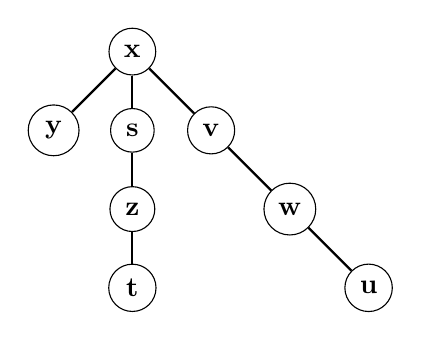
\begin{tikzpicture}
	
	\node[shape=circle,draw=black] (x) at (0, 0)     {\textbf{x}};
	\node[shape=circle,draw=black] (y) at (-1, -1) 	 {\textbf{y}};
	\node[shape=circle,draw=black] (s) at (0, -1) 	 {\textbf{s}};
	\node[shape=circle,draw=black] (v) at (1, -1) 	 {\textbf{v}};
	\node[shape=circle,draw=black] (w) at (2, -2) 	 {\textbf{w}};
	\node[shape=circle,draw=black] (u) at (3, -3) 	 {\textbf{u}};
	\node[shape=circle,draw=black] (z) at (0, -2) 	 {\textbf{z}};
	\node[shape=circle,draw=black] (t) at (0, -3) 	 {\textbf{t}};
	
	\path[-, thick] (x) edge (y);
	\path[-, thick] (x) edge (s);
	\path[-, thick] (x) edge (v);
	\path[-, thick] (w) edge (u);
	\path[-, thick] (w) edge (v);
	\path[-, thick] (z) edge (s);
	\path[-, thick] (z) edge (t);

\end{tikzpicture}
\end{figure}
\item After adding (u,y,3):
\begin{figure}[H]
\centering
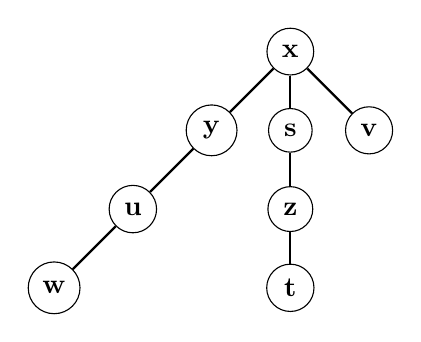
\begin{tikzpicture}
	
	\node[shape=circle,draw=black] (x) at (0, 0)     {\textbf{x}};
	\node[shape=circle,draw=black] (y) at (-1, -1) 	 {\textbf{y}};
	\node[shape=circle,draw=black] (s) at (0, -1) 	 {\textbf{s}};
	\node[shape=circle,draw=black] (v) at (1, -1) 	 {\textbf{v}};
	\node[shape=circle,draw=black] (w) at (-3, -3) 	 {\textbf{w}};
	\node[shape=circle,draw=black] (u) at (-2, -2) 	 {\textbf{u}};
	\node[shape=circle,draw=black] (z) at (0, -2) 	 {\textbf{z}};
	\node[shape=circle,draw=black] (t) at (0, -3) 	 {\textbf{t}};
	
	\path[-, thick] (x) edge (y);
	\path[-, thick] (x) edge (s);
	\path[-, thick] (x) edge (v);
	\path[-, thick] (w) edge (u);
	\path[-, thick] (u) edge (y);
	\path[-, thick] (z) edge (s);
	\path[-, thick] (z) edge (t);

\end{tikzpicture}
\end{figure}
\item After adding (w,z,-1):
\begin{figure}[H]
\centering
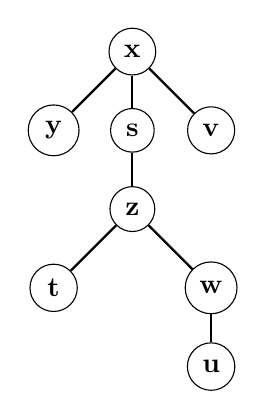
\begin{tikzpicture}
	
	\node[shape=circle,draw=black] (x) at (0, 0)     {\textbf{x}};
	\node[shape=circle,draw=black] (y) at (-1, -1) 	 {\textbf{y}};
	\node[shape=circle,draw=black] (s) at (0, -1) 	 {\textbf{s}};
	\node[shape=circle,draw=black] (v) at (1, -1) 	 {\textbf{v}};
	\node[shape=circle,draw=black] (w) at (1, -3) 	 {\textbf{w}};
	\node[shape=circle,draw=black] (u) at (1, -4) 	 {\textbf{u}};
	\node[shape=circle,draw=black] (z) at (0, -2) 	 {\textbf{z}};
	\node[shape=circle,draw=black] (t) at (-1, -3) 	 {\textbf{t}};
	
	\path[-, thick] (x) edge (y);
	\path[-, thick] (x) edge (s);
	\path[-, thick] (x) edge (v);
	\path[-, thick] (w) edge (z);
	\path[-, thick] (u) edge (w);
	\path[-, thick] (z) edge (s);
	\path[-, thick] (z) edge (t);

\end{tikzpicture}
\end{figure}
\end{itemize}
\subsection*{d}
Yes. Since we construct a minimum spanning tree, we can use the edges of it. So, the shortest path from s to t is szt has weight -3+3=0.
\section*{Answer 6}
\subsection*{a}
13 vertices, 12 edges, height is 4.
\subsection*{b}
Post-order traversal: w, s, m, t, q, x, n, y, u, z, v, r, p.\\
\subsection*{c}
In-order traversal: s, w, q, m, t, p, x, u, n, y, r, v, z.\\
\subsection*{d}
Pre-order traversal: p, q, s, w, t, m, r, u, x, y, n, v, z.\\
\subsection*{e}
No. In a full binary tree every node has two children except the ones at height 0.
\subsection*{f}
No since x:41 should be in the sub-tree of p:42.
\subsection*{g}
By the definition on page 748, in a full m-ary tree, every internal vertex has exactly m children. Let N be the number of vertices.
$$N=1+3+3^2+3^3+...=\sum_{k=0}^h3^k=\dfrac{3^{h+1}-1}{3-1}=\dfrac{3^{h+1}-1}{2}$$
\subsection*{h}
\begin{figure}[H]
	\centering
	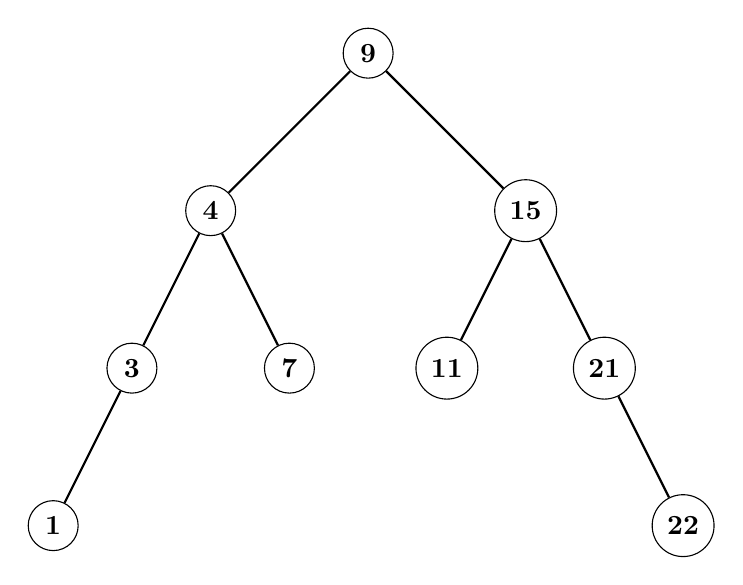
\begin{tikzpicture}
	
	\node[shape=circle,draw=black] (9) at (0, 6)     {\textbf{9}};
	\node[shape=circle,draw=black] (4) at (-2,4) 	 {\textbf{4}};
	\node[shape=circle,draw=black] (15) at (2,4) 	 {\textbf{15}};
	\node[shape=circle,draw=black] (3) at (-3,2) 	 {\textbf{3}};
	\node[shape=circle,draw=black] (7) at (-1,2) 	 {\textbf{7}};
	\node[shape=circle,draw=black] (11) at (1,2) 	 {\textbf{11}};
	\node[shape=circle,draw=black] (21) at (3,2) 	 {\textbf{21}};
	\node[shape=circle,draw=black] (1) at (-4,0) 	 {\textbf{1}};
	\node[shape=circle,draw=black] (22) at (4,0) 	 {\textbf{22}};
	
	\path[-, thick] (9) edge (4);
	\path[-, thick] (9) edge (15);
	\path[-, thick] (4) edge (3);
	\path[-, thick] (4) edge (7);
	\path[-, thick] (15) edge (11);
	\path[-, thick] (15) edge (21);
	\path[-, thick] (3) edge (1);
	\path[-, thick] (21) edge (22);
	
	
	\end{tikzpicture} 	
\end{figure}
\subsection*{i}
For 2: 9, 4, 3, 1. Unsuccessful search.\\
For 22: 9, 15, 21, 22. Successful search.
\subsection*{j}
\begin{figure}[H]
	\centering
	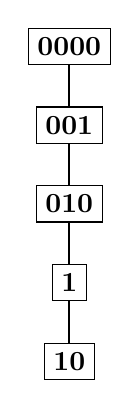
\begin{tikzpicture}
	
	\node[shape=rectangle,draw=black] (0000) at (0, 6)     {\textbf{0000}};
	\node[shape=rectangle,draw=black] (001) at (0,5) 	 {\textbf{001}};
	\node[shape=rectangle,draw=black] (010) at (0,4) 	 {\textbf{010}};
	\node[shape=rectangle,draw=black] (1) at (0,3) 	 {\textbf{1}};
	\node[shape=rectangle,draw=black] (10) at (0,2) 	 {\textbf{10}};
	
	\path[-, thick] (0000) edge (001);
	\path[-, thick] (010) edge (001);
	\path[-, thick] (010) edge (1);
	\path[-, thick] (1) edge (10);
	
	
	\end{tikzpicture} 	
\end{figure}
\subsection*{k}
For 001: 0000, 001. Successful search. \\
For 011: 0000, 001, 010, 1. Unsuccessful search.
\subsection*{l}
First tree: 
\begin{figure}[H]
	\centering
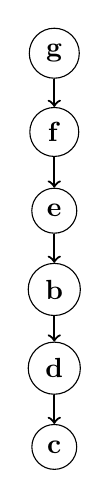
\begin{tikzpicture}
	
	\node[shape=circle,draw=black] (g) at (0, 0)     {\textbf{g}};
	\node[shape=circle,draw=black] (f) at (0, -1) 	 {\textbf{f}};
	\node[shape=circle,draw=black] (e) at (0, -2) 	 {\textbf{e}};
	\node[shape=circle,draw=black] (b) at (0, -3) 	 {\textbf{b}};
	\node[shape=circle,draw=black] (d) at (0, -4) 	 {\textbf{d}};
	\node[shape=circle,draw=black] (c) at (0, -5) 	 {\textbf{c}};
	
	\path[->, thick] (g) edge (f);
	\path[<-, thick] (e) edge (f);
	\path[->, thick] (e) edge (b);
	\path[<-, thick] (d) edge (b);
	\path[->, thick] (d) edge (c);
	

\end{tikzpicture}
\end{figure}
Second tree:
\begin{figure}[H]
	\centering
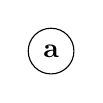
\begin{tikzpicture}
	
	\node[shape=circle,draw=black] (a) at (0, 0)     {\textbf{a}};

\end{tikzpicture}
\end{figure}
\end{document}

​

